\documentclass[twocolumn,aps,prx,amsmath,amssymb,longbibliography]{revtex4-2}
\usepackage{graphicx}
\usepackage{dcolumn}
\usepackage{bm}
\usepackage{amsfonts}
\usepackage{xcolor,tabu}
\usepackage{multirow}
\usepackage{amsthm}
\usepackage{textcomp}
\usepackage{tikz}
\usepackage[colorlinks=true,
            linkcolor=blue,
            urlcolor=blue,
            citecolor=blue]{hyperref}
\hypersetup{bookmarksopen=true}
\usepackage{xr}


% \author{Zhengyang Liu, Wei Zeng, Xiaolei Ma, Xiang Cheng}
%\email{liux3141@umn.edu}
% \affiliation{Department of Chemical Engineering and Materials Science, University of Minnesota, Minneapolis, Minnesota 55455, USA}
\date{\today}

\begin{document}
\title{Density Fluctuations and Energy Spectra of 3D Bacterial Suspensions\\
        Supplemental Material}


\author{Zhengyang Liu}
%\email{liux3141@umn.edu}
\author{Wei Zeng}
\author{Xiaolei Ma}
\author{Xiang Cheng}


\affiliation{Department of Chemical Engineering and Materials Science, University of Minnesota, Minneapolis, MN 55455, USA}


\maketitle

% What is needed in this supplemental material?
% - all the methods I have used in the main text, including:
%   - bacterial samples
%   - microscopy
%   - GNF
%   - PIV
%   - cross-correlation
%   - energy spectra
% - Justification of methods and parameter choices
%   - two GNF methods
%   - local density flucution duration (10 frames)
%   - kinks in energy spectra curves
%   - normalize GNF at small length scale
%   - does image contrast matter?
% - Movie
%   - vigorous bacterial turbulence
%   - PIV overlay

\section{Experiment details}
\subsection{Light-powered \textit{E. coli}}
We introduce a light-driven transmembrane proton pump, proteorhodopsin (PR), to wild-type \textit{E. coli} (BW25113) by transforming the bacteria with plasmid pZE-PR encoding the SAR86 $\gamma$-proteobacterial PR-variant (Walter 2007). The activity of PR is correlated with the intensity of light. Thus, we can control the swimming speed of bacteria using light of different intensities. In our experiments, we use high-intensity light, which saturates the light response of bacteria. The average swimming speed of bacteria is fixed at $v_0 = 15 \pm 3$ $\mu$m/s in the dilute limit.

The bacteria are cultured at 37 \textcelsius{} with a shaking speed at 250 rpm for 14-16 hours in terrific broth (TB) [tryptone 1.2\% (w/w), yeast extract 2.4\% (w/w), and glycerol 0.4\% (w/w)] supplemented with 0.1 g/L ampicillin. The culture is then diluted 1: 100 (v: v) in fresh TB and grown at 30 \textcelsius{} for 6.5 hours. PR expression is triggered by supplementing the culture medium with 1 mM isopropyl $\beta$-D-thiogalactoside and 10  $\mu$M ethanolic all-trans-retinal in the mid-log phase (3 hours after the dilution).

The bacteria are harvested by gentle centrifugation ($800g$ for 5 min). After discarding the culture medium in the supernatant, we resuspend bacteria with DI water. The resuspended suspension is then centrifuged again at $800g$ for 5 min, and finally adjusted to the target concentration for experiments.

\subsection{Sample preparation and microscopy}

To prepare the sample for microscopy, we construct a seal chamber made of glass slides (25 mm $\times$ 75 mm) and coverslips (18 mm $\times$ 18 mm). We first glue (NOA 81, Norland, NJ) two coverslips on a glass slide, side-by-side, leaving a 3-mm separation between the two coverslips. We then cover the 3-mm separation with another coverslip to form a channel. We then pipette bacterial suspensions into the channel. Finally, we seal the two ends of the channel using UV glue (NOA 76, Norland, NJ) to form a sealed chamber.

Images of the bacterial suspensions are taken 50 $\mu$m above the bottom surface of the sealed chamber by a Nikon Ti-E inverted microscope using the bright field mode and a 20$\times$ (NA 0.5) objective. The field of view is 420 $\times$ 360 \textmu m$^2$. All videos are recorded at 30 frames per second using a sCMOS camera.

%%\subsubsection{Linear relation between intensity and density}
%%In the low attenuation limit (small thickness and weak absorptivity), $I=I_0-\epsilon$ where $\epsilon\ll I_0$:
%%\begin{equation}
%%  \log \frac{I_0}{I} = \log \frac{I_0}{I_0 - \epsilon} \approx \frac{\epsilon}{I_0} \sim c
%%\end{equation}
%%\begin{equation}
%%I = I_0 - \epsilon \sim c
%%\end{equation}
%%where $I_0$ is the original light intensity, $I$ is the transmission light intensity, $\epsilon$ is the attenuated light intensity, which is much smaller than the original light intensity.

%%%%%%%%%%%%%%%%%%%%%%%%%%%%%%%%%%%%%%%%%%%%%%%%%%%%%%%%%%%%%%%%%%%%%%%%%%%%%%%%%%%%%%%%%%%

\begin{figure*}[!]
\begin{center}
\includegraphics[width=0.8\textwidth]{figures/GNF-calculation/v1.pdf}
\caption[GNF calculations]
{
\textbf{GNF calculations.}
(a) Varying subsystem sizes.
(b) Multiple seeds of subsystems for spatial average.
}
\label{GNF-calculation}
\end{center}
\end{figure*}


\section{Image analysis details}
\subsection{Calculation of density fluctuations}
\label{sec:GNF-calculations}
% \subsubsection{Two different methods}
%
% Two different methods have been used to calculate number density fluctuations in experiments \cite{Narayan2007,Aranson2008}. Both methods divide a large system into small subsystems of fixed size $l$. The first method calculates the mean particle number $N$ and the standard deviation of particle number $\Delta N$ in each subsystem over time first and then average $N$ and $\Delta N$ spatially over all the subsystems, i.e., temporal variance followed by spatial average (the TVSA method) \cite{Narayan2007}. The second method reverses the procedure, which calculates $N$ and $\Delta N$ over all the small subsystems in one frame first and then takes an temporal average over all frames, i.e., spatial variance followed by temporal average (the SVTA method) \cite{Aranson2008}.
%
% \textcolor{red}{I don't understand the purpose of this paragraph. Do you like to argue that the two methods are the same for our system? But this is not correct.} Ref. XX showed that when a system is homogeneous, where spatial and temporal correlations are small compared with the system size and experiment duration, the two methods lead to the same results. Bacterial suspensions used in our study have correlation lengths smaller than the system size ($\sim 140$ \textmu m), and is thus spatially homogeneous. When the duration of experimental videos is longer than the autocorrelation times, the system can be also regarded as being temporally homogeneous as well.
%
% In our experiments, we correlate image pixel intensity with local particle density. Nevertheless, the non-uniformity of light illumination induces temporally stable intensity variations even without bacterial suspensions. Such intrinsic intensity variations would lead systematic errors in density fluctuations when the second method of SVTA is used. Thus, we adopt the TVSA method, which is insensitive to the temporally stable intensity variations and avoids the potential errors due to the non-uniform light illumination.




%%%%%%
\subsubsection{Convert intensity to density}
In Fig.~1d, we show that under the same illumination and imaging condition, the density and average pixel intensity follow approximately a linear relation, which can be expressed as suggests:
\begin{equation}
  \label{eq:phi-I-relation}
  \phi = a + bI
\end{equation}
where $\phi$ is the volume fraction of bacterial suspensions, $I$ is the average pixel intensity in a window, $a$ and $b$ are constants under the same illumination and imaging conditions. The number of bacteria in a given subsystem with side length $l$ and thickness $d$ can be calculated as
\begin{equation}
  \label{eq:n}
  N = \frac{\phi l^2d}{V_b}
\end{equation}
where $V_b$ is the volume of a single bacterium. Take the standard deviation of both sides of Eq.~\ref{eq:n}, we get
\begin{equation}
  \Delta N = \frac{|b|d}{V_b} l^2\Delta I
\end{equation}
where $\Delta$ stands for taking the standard deviation over time. Over different length scales and volume fractions, $\frac{|b|d}{V_b}$ is a constant. Thus, we use $l^2\Delta I$ as $\Delta N$ in all the figures.

%%%%%%%%

\begin{figure}[t]
	\begin{center}
		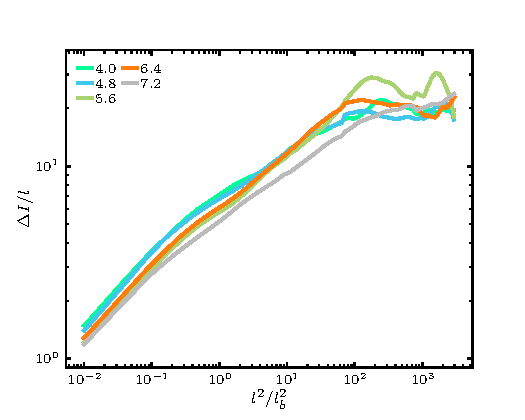
\includegraphics[width=0.46\textwidth]{Figures/GNF-normalization/same-illumination.pdf}
		\caption[Density autocorrelation]
		{
			\textbf{GNF curves at various volume fractions under same illumination and imaging conditions.}
		}
		\label{fig:same-conditions}
	\end{center}
\end{figure}

%% To illustrate the effect of changing imaging conditions, we measure the GNF of the same sample, under the same illumination, and use both 1 ND filter and 2 ND filter under the objective to dimmer the light that goes to the camera. Note that we have to use at least one filter to avoid over exposure of the camera. The result is shown in Fig.~\ref{fig:filter-effect}, where all the four runs with 2 filters falls into a bundle, where as the run with only one filter clearly lies out of the bundle. Despite the big difference in the magnitude, the overall length scale dependence is quite similar, suggesting that measuring GNF using light intensity is valid.

\subsubsection{Density fluctuations at different length scales}

Equipped with the relation between $\Delta N$ and $\Delta I$, we now calculate the density fluctuations at different length scales (using $l^2\Delta I$). We first crop square-shape subsystems of various sizes from the original image time series, as shown in Fig.~\ref{GNF-calculation}a. For each size $l$, a standard deviation of the light intensity are calculated over 50 frames (1.67 s). To improve statistics, we choose 20 subsystems of the same size evenly distributed in the field of view and obtain an averaged standard deviation of mean intensity $\Delta I$ (Fig.~\ref{GNF-calculation}b). This averaged $\Delta I$ is then multiplied by $l^2$ and is used as the density fluctuations $\Delta N$.

% \textcolor{red}{Please rewrite/reorganize this section. I combine this session with the session on the normalization of GNF. The two sessions together allow you to convert $I$ into $N$ eventually.}
% Using the TVSA method, we first crop square-shape subsystems of various sizes from the original image time series, as shown in Fig.~\ref{GNF-calculation}a. For each size $l$, a standard deviation of the light intensity $\Delta I$ are calculated over time. \textcolor{red}{What you directly measure is the image intensity. I suggest we use $\Delta I$ and $I$ first and state clearly how $\Delta I$ and $I$ are related to $\Delta N$ and $N$ at the end.} To improve statistics, we choose 20 different subsystems of the same size evenly distributed in the field of view and obtain an average $\Delta I$ and $I$  (Fig.~\ref{GNF-calculation}b). We vary the subsystem size $l$ from 10 \textmu m to 30 \textmu m, \textcolor{red}{from 10 to 30 um? It seems to be a very small range.} and examine the temporal variations of image intensity $\Delta I_{i}(l)$ in the $i^{th}$ frame for subsystem size $l$. The temporal variations are then averaged in space (over $i$) to give the final $\Delta I$. \textcolor{red}{I am confused that if $i$ is the number of frame, why is it an average of space?} Since $I$ is linearly proportional to bacterial volume fraction $\phi$. $\Delta I \sim \Delta \phi$
% Then number fluctuations in the system is captured by the dependence of $\Delta N_{j}$ on $l_j$. In an equilibrium system, $\Delta N_{j}\propto l_j$ (this follows from $\Delta N_{j}\propto \sqrt{N_j}$ and $N_j\propto l_j^2$).
% Thus, the deviation from $\Delta N_{j}\propto l_j$ quantifies the giant number fluctuation in the system.
% In the main paper, we plot $\Delta N_{j}/l_j$ as a function of $l_j^2/l_b^2$, where $l_b$ is the length scale of single bacterial body length, chosen to be 3 \textmu m.
% To be consistent with the notations in literatures, we get rid of the subscript $j$, and write $l_j$ as $\sqrt{N}$.
% Note that the subscript $j$ denotes different choices of box sizes.

% Without a more careful calibration, we are not able to obtain the exact number of particles using this Beer's law based method. Fortunately, the calculations of GNF does not require the exact number, but only the relative number. In the main paper, we show that the volume fractions $\phi$ and average pixel intensities $I$ follow a pretty linear relation. Such a relation entails that $\Delta I \propto \Delta N$, which is followed by $\Delta I/\sqrt N \propto \Delta N/\sqrt N$. The proportionality allows us to get the scaling exponents of $\Delta N/\sqrt N$ against $N$, without having to measure the exact particle numbers.


\subsubsection{Normalization}

For optimal image qualities, we used different exposure times when acquiring the data. However, such difference prevents us from comparing $\Delta N$ at different volume fractions, since exposure time changes the overall magnitude of the image intensity fluctuations, independent of the fluctuations in the bacterial sample. In order to compare the magnitude of GNF across different volume fractions, and more importantly compare GNF with energy spectra, we need to normalize the GNF curves obtained at different illumination and imaging conditions, so that they reflect the actual relative magnitude independent of illumination and imaging conditions. To do it, we use the same illumination and imaging conditions to take videos of bacterial suspensions at various volume fractions where we control all the imaging parameters strictly.  The results are shown in Fig.~\ref{fig:same-conditions}, where all the curves are very close at small length scale, and show deviation at large length scales. This observation is intuitive: small scale density fluctuations is determined primarily by single cell dynamics and is not a strong function on volume fractions. In the main text, we normalized all the GNF curves at small length scale, by forcing $\Delta N_{0.3l_b}=1$.


\subsection{Particle image velocimetry (PIV)}

2D in-plane velocity fields are extracted by Particle Image Velocimetry (PIV) analysis using openPIV package in Python \cite{Liberzon2020}. %(Fig.~\ref{fig:1}b).
We fix the box size to be 16 $\mu$m, which is larger than the size of a single bacterial body but smaller than the velocity correlation length. A step size of the half of the box size (8 $\mu$m) is used by convention, which sets the spatial resolution of the velocity fields.

\subsection{Energy spectra}
The energy spectra of bacterial suspensions are calculated as follows.

%% \textcolor{red}{Again, we need to show how the calculation is actually performed, instead of the theory behind. For example, we should state how we use FFT on the PIV velocity data and how the results are related to $E(k_x,k_y)$. Finally, we should discuss how $E(k_x,k_y)$ is used to finally get $E(k)$.}
\begin{equation}
E(k_x, k_y) = \frac{\langle u_k(k_x, k_y)u^*_k(k_x, k_y)+v_k(k_x, k_y)v_k^*(k_x, k_y)\rangle}{2A}
\end{equation}
where $E$ is the energy density in $k$ space, $u_k$ and $v_k$ are $k$ space velocity fields, $A$ is the real space area of the system and $^*$ denotes the complex conjugate. The $\langle\cdot\rangle$ denotes an average over multiple images from different times.

The fourier transform of real space velocity $u_k$ and $v_k$ are computed as the following:
\begin{itemize}
  \item apply the built-in Fast Fourier Transform (FFT) function of Python \texttt{numpy.fft} package to the discrete velocity field $v(x, y)$ (from PIV) to get $V_k(k_x, k_y)$
  \item since the FFT is defined as
    $$
    V_k=\sum^{n-1}_{m=0}v_m\exp(-2\pi i \frac{mk}{n})
    $$
    missing the $dx$ counterpart in the continuous Fourier transform, we additionally multiply $d_{step}^2$ to $V_k(k_x, k_y)$ to get the wavenumber domain velocity $v_k(k_x, k_y)$
  \item the wavenumber field $k$ corresponding to $v_k(k_x, k_y)$ is obtained by applying the \texttt{numpy.fft.fftfreq} function. Since the definition of FFT introduces a prefactor $2\pi$ to the wavenumber, an additional $2\pi$ is also multiplied to $k$
\end{itemize}


% This method can be shown to be equivalent to another commonly used formula, which calculates the Fourier transform of real space velocity spatial correlation functions:
% \begin{equation}
% E^1 = \int \langle \boldsymbol{u}(\boldsymbol{r_0}) \boldsymbol{u}(\boldsymbol{r_0}+\boldsymbol{r}) \rangle
% e^{-i\boldsymbol{k}\cdot\boldsymbol{r}} d\boldsymbol{r}
% \end{equation}
%
% \textcolor{red}{it is good to document the following derivation somewhere (maybe in your thesis), but we don't need to show it in the paper.)}
% We show here how they are equivalent by considering one of the velocity componenet $u$. Starting with the definition of $E$
% \begin{equation}
% \begin{split}
% E(k_x, k_y) &= u_k(k_x, k_y)u_k^*(k_x, k_y)\\
% & = \iint u(x, y)e^{-ik_xx}e^{-k_yy}dxdy\left[\iint u(x', y')e^{-ik_xx'}e^{-ik_yy'}dx'dy'\right]^*\\
% & = \iint u(x, y)e^{-ik_xx}e^{-k_yy}dxdy\iint u^*(x', y')e^{ik_xx'}e^{ik_yy'}dx'dy'\\
% & = \iiiint u(x, y)u(x', y')e^{-ik_x(x-x')}e^{-k_y(y-y')}dxdydx'dy'
% \end{split}
% \end{equation}
% here, we change variable and let $x'' = x - x'$ and $y'' = y - y'$ the original expression can be rearranged into
% \begin{equation}
% \begin{split}
% & \iiiint u(x'+x'', y'+y'')u(x', y')e^{-ik_xx''}e^{-k_yy''}d(x'+x'')d(y'+y'')dx'dy'\\
% & = \iint \left[\iint u(x'+x'', y'+y'')u(x', y')dx'dy'\right] e^{-ik_xx''}e^{-k_yy''} d(x'+x'')d(y'+y'')
% \end{split}
% \end{equation}
% using the definition of velocity correlation function (average all possible pairs over available space):
% \begin{equation}
% \langle u(x, y)u(x+x'', y+y'') \rangle = \frac{\iint u(x'+x'', y'+y'')u(x', y')dx'dy'}{\iint dx'dy'}
% \end{equation}
% we obtain
% \begin{equation}
% \iint dx'dy'\iint \langle u(x, y)u(x+x'', y+y'') \rangle e^{-ik_xx''}e^{-k_yy''} dx''dy''
% \end{equation}
% the first integration is the available space size of velocity field, in this case the system area $A$. Thus,
% \begin{equation}
% E(k_x, k_y) = E^1(k_x, k_y)
% \end{equation}

\begin{figure}[t]
	\begin{center}
		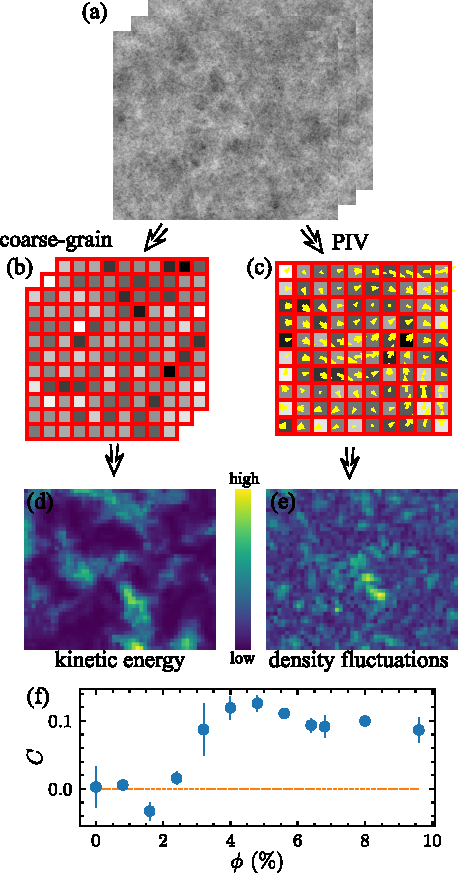
\includegraphics[width=0.46\textwidth]{Figures/local-correlation/v1.pdf}
		\caption[Density autocorrelation]
		{
			Diagram showing the procedures of calculating local coupling between density fluctuations and kinetic energy.
		}
		\label{fig:coupling-calculation}
	\end{center}
\end{figure}

\subsection{Correlation of local density fluctuations and kinetic energies}

%% \textcolor{red}{We need more details. In addition to the definition of the correlation function, we need to show how the density fluctuations and kinetic energies are calculate at $l = 2.5l_b$, staring from pixel image intensity and velocity fields at 8 um spacing.}

Here we show the procedures of calculating the local coupling between density fluctuations and kinetic energy. When calculating the local density fluctuations, we want to measure the instantaneously change of density instead of a steady-state scaling. Thus, we choose the length of video for this calculation to be within the autocorrelation time of density (or more accurately, average pixel intensity) variations, which is typically around 2s, or 60 frames, as shown in Fig.\ref{fig:spatiotemporal-correlations}. We also want to include as many frames as we can instead of using adjacent frame, in order to suppress the effects from random fluctuations of image intensities, the nature of optical imaging. Thus, we used 10 frames for the local density fluctuation calculation. We don't expect the result to be much different when varying this number from 5 to 20.

As shown in Fig.~\ref{fig:coupling-calculation}, we first take 10 frames $F_i(\bm{r})$ of consecutive images, where $i=1, 2, ..., 10$. All the 10 frames are coarse-grained by binning $25\times 25$ px$^2$ ($8\times8$ $\mu$m$^2$) windows into a single pixel $f_i(\bm{r})$, as shown in Fig.~\ref{fig:coupling-calculation}b. PIV algorithm is then applied on the first two images to obtain a representative velocity field $v{\bm{r}}$, as in Fig.~\ref{fig:coupling-calculation}c. Since the PIV analysis is done at a step size of 25 pixel, the coarse-graining procedure produces images with dimensions the same as the velocity fields obtained from PIV. We then take the standard deviation of the pixel intensity at each spot over 10 frames to obtain a field of density fluctuations, $\delta N(\bm{r}) = \sqrt{\langle(f_i-\langle f_i\rangle)^2\rangle}$, shown in Fig.~\ref{fig:coupling-calculation}d. The kinetic energy field is obtained by taking square of the magnitudes of PIV result and then divide it by 2, $E_k(\bm{r})=\langle v(\bm{r})^2 / 2 \rangle$, as shown in Fig.~\ref{fig:coupling-calculation}e. Finally, the normalized correlaiton between $\Delta N(\bm{r})$ and $E_k(\bm{r})$ is calculated as
\begin{equation}
  \Delta N\star E_k = \frac{\langle(\Delta N-\overline{\Delta N})(E_k-\overline{E_k})\rangle}{\sigma_{\Delta N}\sigma_{E_k}}
\end{equation}

$\star$ is the operator standing for cross correlation, $\bar\cdot$ means taking the mean, $\sigma$ means the standard deviation, and $\langle\cdot\rangle$ denotes taking the average of all scalars in an array. The cross correlation quantifies the similarity between arrays $N$ and $E_k$. The resulting number takes value from -1 to 1.

\subsection{Density fluctuations in the transient state}

The density fluctuations in transient state is calculated using the same method as the steady state. The procedures described in Sec.~\ref{sec:GNF-calculations} is repeated every 50 frames in videos where the whole process of bacterial activity rising is recorded. Why 50 frames? It is about the length of correlation time, so we expect sound statistics from it. It is also short compared to the whole process of $\alpha$ rising (60 s, or 1800 frames), so it can also provide good temporal resolution to monitor the kinetic process.




% \textcolor{red}{This session is necessary. I have not worked on the revision of the session yet though.}



% We first calculate the autocorrelation functions of density. The basic principle of this calculation is to shift a time series of density at varying steps and calculate the matching between the original series and the shifted series, using the cross correlation scheme as in Eq.~\ref{eq:cross-correlation}. In Fig.~\ref{fig:density-autocorrelation}, we plot the autocorrelation function of density at various volume fractions, covering the range studied in this work. We notice that low volume fraction suspensions display a longer correlation time. The smallest correlation time, according to this measurement, is around 1 second, which corresponds to 30 frames in our videos. Thus, we choose 10 frames as the video length for calculating the local density fluctuations, which is much smaller than the correlation time but still has many enough frames to suppress the random flucutations from imaging.

% \begin{figure}[!]
% \begin{center}
% \includegraphics[width=0.7\textwidth]{figures/density-autocorrelation/v1.pdf}
% \caption[Density autocorrelation]
% {
% \textbf{Density autocorrelation.}
% }
% \label{fig:density-autocorrelation}
% \end{center}
% \end{figure}

% \begin{figure}[t]
% \begin{center}
% 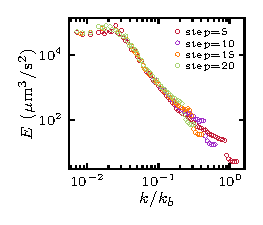
\includegraphics[width=0.46\textwidth]{Figures/kinks-in-energy-spectra/v1.pdf}
% \caption[Density autocorrelation]
% {
% \textbf{Energy spectra of the same active turbulence, measured at different PIV step size.}
% }
% \label{fig:kink}
% \end{center}
% \end{figure}



%%\subsection{Kinks in energy spectrum curves}
%%At high $k$ limit, the energy spectra in Fig.~4 show kinks. We show here that such kinks are due to the step size in PIV analysis and in unavoidable when approaching very small length scales. We also note that we choose the smallest step to be the length of single bacterium, so that all lengths above that scale do not show kink.



%%Fig.~\ref{fig:kink} shows the energy spectra of the same sample, but using PIV with different step sizes ranging from 5 to 20 pixels (corresponding to 1.5 to 6 $\mu$m, or 0.5 to 2 $l_b$). Despite the different step sizes used in PIV, the majority of the 4 curves agree with each other well. Kinks happen in the large $k$ limit, and the locations of kinks move towards larger $k$ as step size getting smaller, in consistency with our expectation.

%%\begin{figure}[!]
%%\begin{center}
%%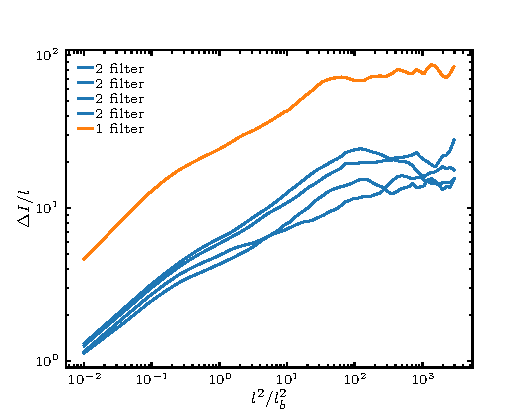
\includegraphics[width=0.7\textwidth]{Figures/GNF-normalization/different-filters.pdf}
%%\caption[Density autocorrelation]
%%{
%%\textbf{GNF curves of the same active turbulence measured with 1 or 2 ND filters below the objective. This is a test experiment showing the effect of imaging condition on the magnitude of GNF curves.}
%%}
%%\label{fig:filter-effect}
%%\end{center}
%%\end{figure}




%%\textcolor{red}{We probably need to document the results somewhere in case referees ask questions, but we don't need to show it in the paper.}

%%\subsection{Does image contrast matter?}

%%Our GNF measurement depends strongly on the image pixel intensities. A natural question is, if we do a simple manipulation of the image, such as autocontrast, would the GNF extracted from the image different? Fig.~\ref{fig:image-contrast} shows the GNF calculation on the same image sequence, but adjusted to different degree of contrast, as shown in Fig.~\ref{fig:image-contrast}a and b. The GNF results are shown in Fig.~\ref{fig:image-contrast}c, the two sequences give rise to exactly the same GNF curve. Note that the normalization described in the previous section is applied here. Otherwise, the magnitude of the curves would be different, while the overall trends are exactly the same.

%%\begin{figure}[!]
%%	\begin{center}
%%		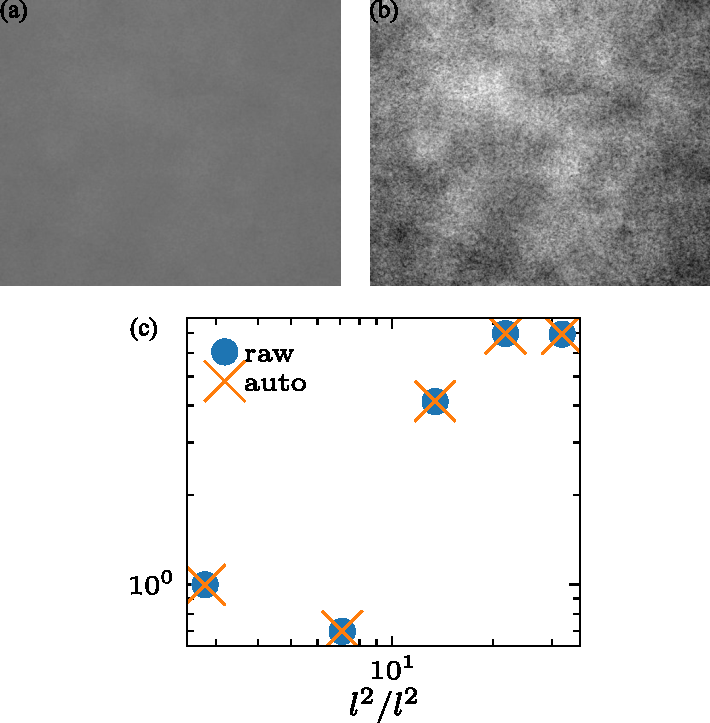
\includegraphics[width=0.7\textwidth]{Figures/image-contrast/v1.pdf}
%%		\caption[Density autocorrelation]
%%		{
%%			\textbf{Test GNF calculation on the same image with different contrast.}
%%			(a) Raw image.
%%			(b) Autocontrasted image.
%%			(c) GNF results.
%%		}
%%		\label{fig:image-contrast}
%%	\end{center}
%%\end{figure}


% \newpage
%
% \section{Supplementary videos}
% Find in ``demo'' folder.
% \subsection{Bacterial turbulence}
% 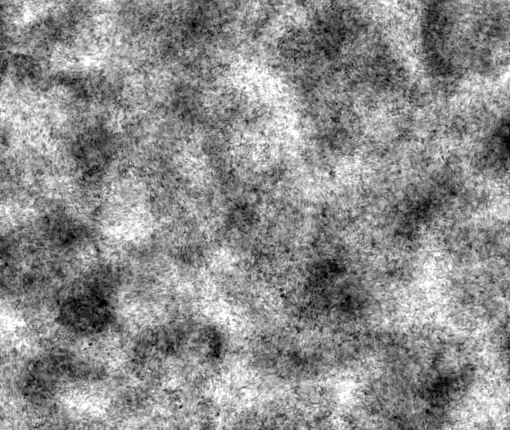
\includegraphics[width=0.5\textwidth]{Figures/video-snapshot/t.jpg}
% \subsection{PIV overlay}
% 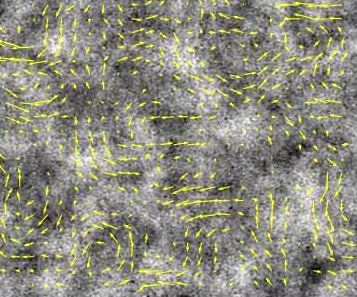
\includegraphics[width=0.5\textwidth]{Figures/video-snapshot/piv.jpg}

\bibliographystyle{apsrev4-2}
\bibliography{../correlation}




\end{document}


\end{document}
